\section{Usability Test}
\label{common:sec:usability_test}
As stated in the motivation, quality assurance through testing of the system is required. Therefore a usability test was conducted in order to measure the current usability of the GIRAF platform as a whole, as well as of the individual parts of the platform. Furthermore, the next wave of developers will immediately be able to start correcting the found usability issues.

\subsection{Approach}
The test group consists of the five contact persons. We assess that they, as a test group, are representative. We base this on them being a mix of educators and teachers, with varying computer skills.

They have prior knowledge about the overall idea of the GIRAF platform, and although some of the contact persons had previously informally used some aspects or parts of the system, they had not been exposed to the platform as a whole, and therefore still are of value.

The invitation sent to the test persons can be found in \ref{appendice:usability_test}.\\

The Instant Data Analysis (IDA) method for usability is chosen. A traditional video analysis method could be used, but since IDA is designed for small test groups, this approach is used. \cite{usability:ida}

\subsubsection*{Setup}
The usability test is divided into two tests: A test of three user applications, and a test of two administrative applications. 
The user applications are: The launcher, PARROT, and WOMBAT. The administrative applications are: The Oasis app and the Savannah web application.
Each test is assigned a team to accommodate the need to run two tests simultaneously.
The teams are made with respect to the criteria of the Instant Data Analysis process.\\
Each team consisted of:

\begin{itemize}
	\item 1 x Test Coordinator
	\item 1 x Test Monitor
	\item 1 x Data Logger
	\item 2 x Observers
\end{itemize}

The usability lab at Aalborg University is designed with two rooms for usability testing and a control room to observe and record the tests.
The two test chambers are assigned a test each and the control room is used to observe both tests as seen in figure \ref{fig:test_setup}.

\begin{figure}[H]
	\centering
		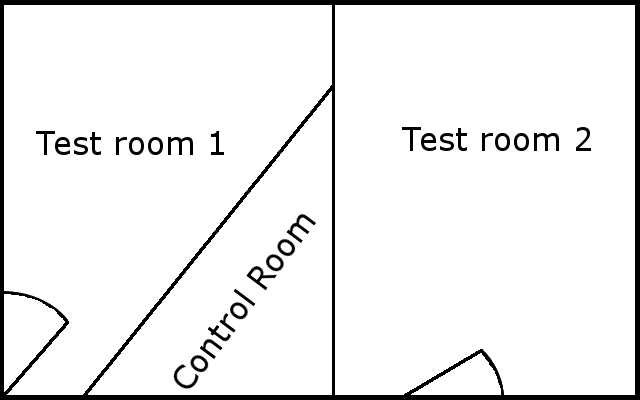
\includegraphics[scale=0.70]{input/images/test_setup.png}
	\caption{An overview of the usability lab at Cassiopeia, Department of Computer Science, Aalborg University.}
	\label{fig:test_setup}
\end{figure}

\subsubsection*{Execution}

\begin{figure}[H]
	\centering
		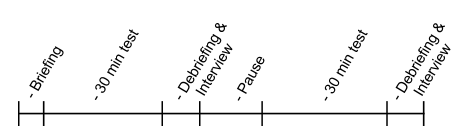
\includegraphics[scale=0.70]{input/images/usability_testschedule.png}
	\caption{The schedule of the usability test.}
	\label{fig:usability_testschedule}
\end{figure}

The tests are conducted according to the schedule in \autoref{fig:usability_testschedule}.

Briefing, debriefing, and questionnaire documents can be found in \autoref {questionnaires}, and the results of the test can be found in \autoref{sec:UseTestRes}.